%!TEX program = xelatex

\documentclass[compress]{beamer}
%--------------------------------------------------------------------------
% Common packages
%--------------------------------------------------------------------------

\definecolor{links}{HTML}{663000}
\hypersetup{colorlinks,linkcolor=,urlcolor=links}

\usepackage[english]{babel}
\usepackage{pgfpages} % required for notes on second screen
\usepackage{graphicx}

\usepackage{multicol}

\usepackage{tabularx,ragged2e}
\usepackage{booktabs}

\usetheme{hri}

% Display the navigation bullet even without subsections
\usepackage{remreset}% tiny package containing just the \@removefromreset command
\makeatletter
\@removefromreset{subsection}{section}
\makeatother
\setcounter{subsection}{1}

\newcommand{\colvec}[2][.8]{%
  \scalebox{#1}{%
    \renewcommand{\arraystretch}{.8}%
    $\begin{bmatrix}#2\end{bmatrix}$%
  }
}

\newcommand{\source}[2]{{\tiny\it Source: \href{#1}{#2}}}

\usepackage{tikz}
\usetikzlibrary{mindmap,backgrounds,positioning,patterns,calc}

\graphicspath{{figs/part4/}}

\title{ROCO318 \newline Mobile and Humanoid Robots}
\subtitle{Part 4 - Wheeled locomotion and kinematics}


\date{}
\author{Séverin Lemaignan}
\institute{Centre for Neural Systems and Robotics\\{\bf Plymouth University}}

\begin{document}

\licenseframe{github.com/severin-lemaignan/module-mobile-and-humanoid-robots}

\maketitle

\begin{frame}{Part 4 -- Wheeled locomotion and kinematics}

For further reading, see:
    
    \begin{itemize}
        \item (Siciliano and Katib, 2008) or chapter 2 from Siegwart and
Nourbakhsh (2004)
    \end{itemize}
\end{frame}

\section{Wheeled robots}

\begin{frame}{Mobile robots with wheels}

    Wheels are the most appropriate solution for most applications.

    $\rightarrow$ The robots are faster and consume less energy.

    Three wheels are \emph{sufficient} and \emph{guarantee stability}.

    \onslide<2->{
        For more than three wheels a flexible suspension is required.
    }
    \begin{columns}
        \begin{column}{0.5\linewidth}

            \onslide<2->{
            Without a flexible suspension, only three wheels would make contact
            with the ground, all other wheels would slip or not contact the
            ground.
            }
            \onslide<3>{
            A large number of wheel types exist

            \begin{itemize}
                \item Selection of wheel type depends on the application.
            \end{itemize}
            }

        \end{column}

        \begin{column}{0.5\linewidth}
            \begin{center}
                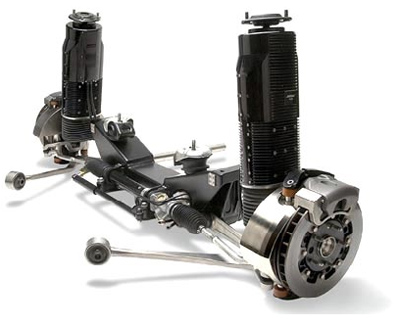
\includegraphics[width=0.8\linewidth]{image1}
            \end{center}
        \end{column}
    \end{columns}

\end{frame}

\begin{frame}{Efficiency of rolling}
    \begin{columns}
        \begin{column}{0.5\linewidth}
            Wheels on rails are almost 100 times more efficient than human walking.

            \begin{itemize}
                \item Robot walking is about 15 times less efficient than human walking.
            \end{itemize}

        \end{column}
        \begin{column}{0.5\linewidth}

            \begin{center}
                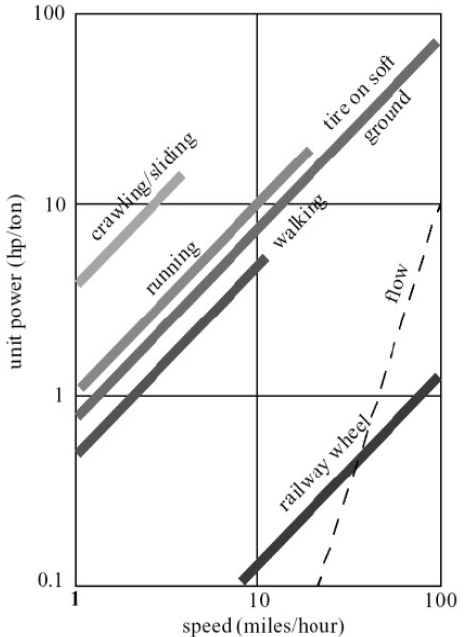
\includegraphics[width=0.8\linewidth]{rolling}
            \end{center}
        \end{column}
    \end{columns}
\end{frame}

\begin{frame}{Three wheel types}

\begin{itemize}
    \item Standard wheel (including the caster wheel).
    \item Omnidirectional wheel (aka \href{http://en.wikipedia.org/wiki/Mecanum_wheel}{Swedish or Mecanum wheel}).
    \item Ball or spherical wheel.
\end{itemize}

\end{frame}

\begin{frame}{Type 1: Standard wheel}


    \only<1>{
        \begin{columns}
            \begin{column}{0.5\linewidth}

                Has two offsets $d$ and $b$.

                The wheel allows steering or not?

                \begin{itemize}
                    \item Can the wheel's orientation be changed or not?
                \end{itemize}

                Is the wheel orientation steered or not?

                \begin{itemize}
                    \item Active steering means that a motor changes the wheel's orientation,
                        passive means that the wheel just follows.
                \end{itemize}

            \end{column}
            \begin{column}{0.5\linewidth}
                \begin{center}
                    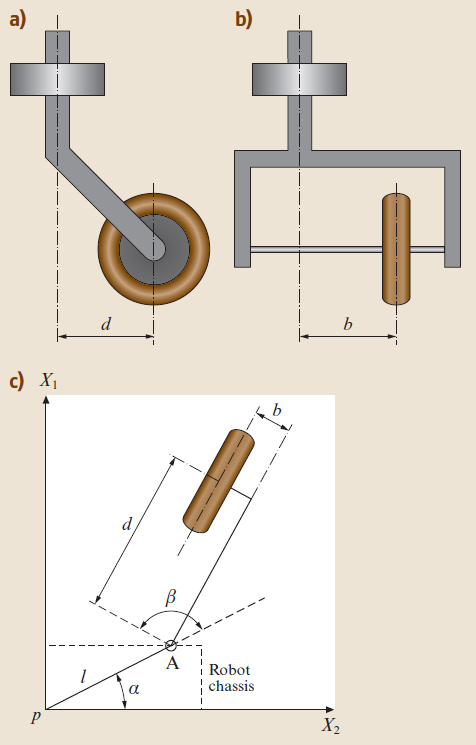
\includegraphics[width=0.8\linewidth]{std_wheel1}
                \end{center}
            \end{column}
        \end{columns}
    }

    \only<2>{

        \begin{columns}
            \begin{column}{0.5\linewidth}

                \textbf{Passive fixed wheel}

                \begin{itemize}
                    \item No motors.
                \end{itemize}

                \textbf{Passive or active caster wheel}

                \begin{itemize}
                    \item The wheel is off-center.
                    \item In the active case, the driving and steering motion is controlled by
                        two motors.
                \end{itemize}

                \textbf{Active wheel that can be oriented}

                \begin{itemize}
                    \item This requires two motors, one for driving and one for steering.
                \end{itemize}
            \end{column}
            \begin{column}{0.5\linewidth}
                \begin{center}
                    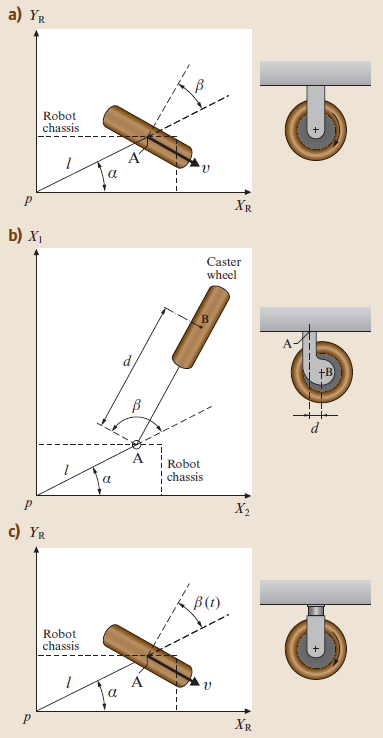
\includegraphics[width=0.7\linewidth]{std_wheel2}
                \end{center}
            \end{column}
        \end{columns}
    }

    \only<3>{
        \textbf{Examples}

    \begin{columns}
        \begin{column}{0.5\linewidth}
            \begin{center}
                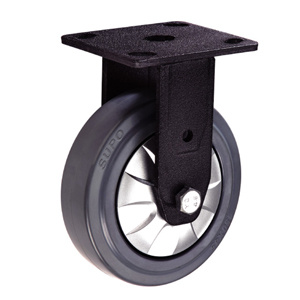
\includegraphics[width=0.8\linewidth]{wheel_ex1}

                Passive fixed wheel
            \end{center}
        \end{column}
        \begin{column}{0.5\linewidth}

            \begin{center}
                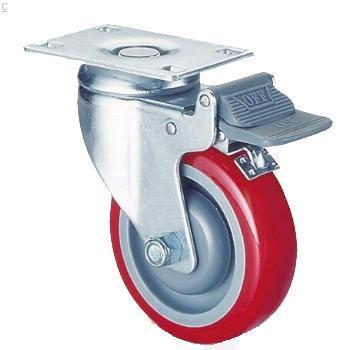
\includegraphics[width=0.8\linewidth]{wheel_ex2}

                Passive caster wheel
            \end{center}
        \end{column}
    \end{columns}
}

\only<4>{
    Standard wheels are most used, but have a \textbf{non-holonomic velocity
constraint}.

\begin{itemize}
    \item Which just means that a wheel can only roll in the direction of the
  wheel and cannot slide sideways.
    \item This constrains what a robot (or vehicle) can do.
\end{itemize}

}

\end{frame}

\begin{frame}{Type 2: Omnidirectional wheel}

    \only<1>{
        \begin{columns}
            \begin{column}{0.5\linewidth}

Omnidirectional wheel (= Swedish or Mecanum wheel).

\begin{itemize}
    \item Three degrees of freedom; rotation around the (motorized) wheel axle,
  around the rollers and around the contact point.
\end{itemize}
            \end{column}
            \begin{column}{0.5\linewidth}
    \begin{center}
        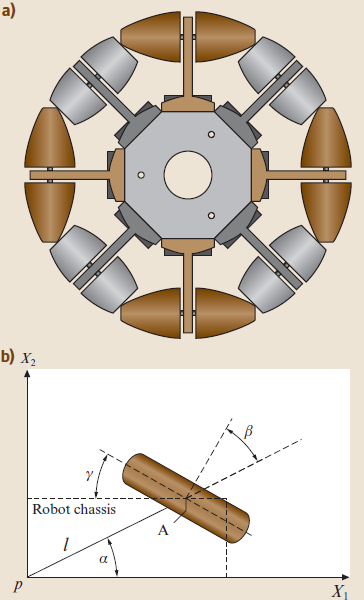
\includegraphics[width=0.8\linewidth]{omniwheel1}
    \end{center}
            \end{column}
        \end{columns}

    }
    \only<2>{
\begin{itemize}
    \item The wheel is designed to let a vehicle move in any direction.
    \item Rollers are mounted at 0 or 45 angles to a line along the plane of
  the wheel.
\end{itemize}

    \begin{center}
        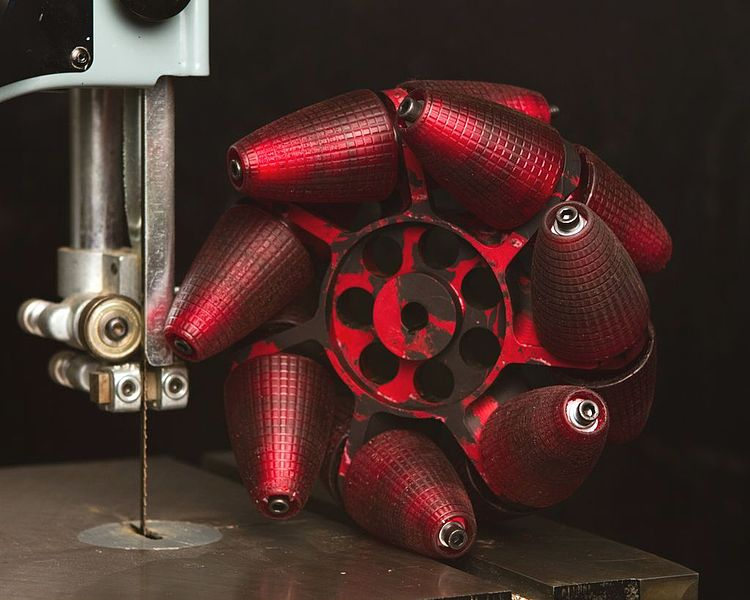
\includegraphics[height=0.4\paperheight]{omniwheel3}
        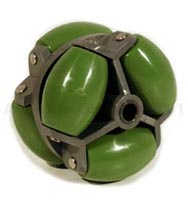
\includegraphics[height=0.4\paperheight]{omniwheel2}

        \source{https://en.wikipedia.org/wiki/Mecanum_wheel}{Wikipedia}
    \end{center}
}

\end{frame}

\begin{frame}{Type 2: Swedish wheel}


    \only<1>{
        \begin{columns}
            \begin{column}{0.6\linewidth}

                Several possible configurations

                \begin{itemize}
                    \item Three motors, and three wheels.
                    \item Four motors and four wheels.
                \end{itemize}

                \begin{center}
                    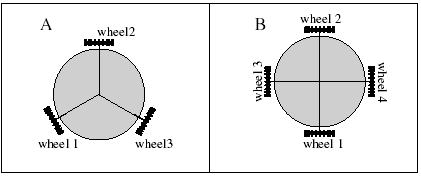
\includegraphics[width=0.8\linewidth]{swedishwheel1}
                \end{center}

            \end{column}
            \begin{column}{0.4\linewidth}

                \begin{center}
                    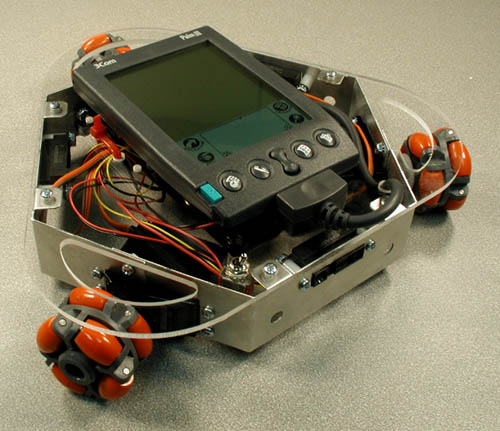
\includegraphics[width=0.8\linewidth]{swedishwheel2}
                \end{center}
            \end{column}
        \end{columns}
    }
    \only<2>{

\begin{itemize}
    \item Four wheels and four motors.

        \begin{center}
            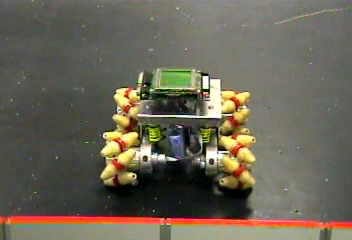
\includegraphics[width=0.45\linewidth]{swedishwheel3}
            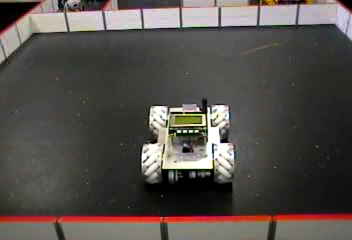
\includegraphics[width=0.45\linewidth]{swedishwheel4}
        \end{center}

    \item Airtrax lift truck
  (\href{http://www.youtube.com/watch?v=IlmKcohyXG0}{video})
\end{itemize}

}
\end{frame}

\begin{frame}{Characteristics of Wheeled Robots and Vehicles}

\emph{Stability of a vehicle is guaranteed with 3 wheels}

\begin{itemize}
    \item centre of gravity must stay within the triangle formed by the ground
  contact point of the wheels.
\end{itemize}

Stability is improved by 4 and more wheels

\begin{itemize}
    \item however, this arrangements are \textbf{hyperstatic} and require a flexible
  suspension system.
\end{itemize}

\pause

Bigger wheels allow to overcome higher obstacles

\begin{itemize}
    \item but they require higher torque and reductions in the gear box.
\end{itemize}

\pause
Most arrangements are \textbf{non-holonomic}: require high control effort.

\pause
Combining actuation and steering on one wheel makes the design complex
and adds additional errors for odometry.

\end{frame}

\begin{frame}{Different Arrangements of Wheels I}

Two wheels

    \begin{tikzpicture} 
        [>=latex,label/.style={align=center,font=\footnotesize},scale=0.8]

        \begin{scope}
            \draw[thick] (0,0) rectangle (3,1);
            \draw[thick, pattern=north east lines] (0.2,0.4) rectangle +(0.6,0.2);
            \draw[rotate around={40:(2.5,0.5)}] (2.5,0.3) rectangle +(0,0.4);
            \draw[thick, rotate around={40:(2.5,0.5)}] (2.2,0.4) rectangle +(0.6,0.2);
        \end{scope}

        \begin{scope}[shift={(5,-0.25)}]
            \coordinate (hatchedwheel) at (0.8,0.5);
            \draw[thick] (0,0) rectangle (1,1.5);
            \draw[thick, pattern=north east lines] (0.2,0.3) rectangle +(0.6,0.2);
            \draw[thick, pattern=north east lines] (0.2,1.2) rectangle +(0.6,-0.2);
        \end{scope}

        \node[align=center, fill=hriSec3Comp!60,font=\footnotesize, text width=3cm, opacity=0.8,text opacity=1, draw,rectangle callout,anchor=pointer,callout relative pointer={(180:1)}] at (hatchedwheel) {Hatched: powered wheels};
    \end{tikzpicture} 


Three wheels

    \begin{tikzpicture} 
        [>=latex,label/.style={align=center,font=\footnotesize},scale=0.8]
        \begin{scope}[shift={(0,-3)}]
            \draw[thick] (0,0) rectangle (3,1.5);
            \draw[thick, pattern=north east lines] (0.2,0.3) rectangle +(0.6,0.2);
            \draw[thick, pattern=north east lines] (0.2,1.2) rectangle +(0.6,-0.2);
            \draw[thick] (2.5,0.75) circle[radius=0.3];
        \end{scope}

        \begin{scope}[shift={(4,-3)}]
            \draw[thick] (0,0) rectangle (3,1.5);
            \draw[thick, pattern=north east lines] (0.2,0.3) rectangle +(0.6,0.2);
            \draw[thick, pattern=north east lines] (0.2,1.2) rectangle +(0.6,-0.2);
            \draw[thick] (0.5,0.5) -- (0.5,1);
            \draw[rotate around={40:(2.5,0.75)}] (2.5,0.55) rectangle +(0,0.4);
            \draw[thick, rotate around={40:(2.5,0.75)}] (2.2,0.65) rectangle +(0.6,0.2);
        \end{scope}

        \begin{scope}[shift={(8,-3)}]
            \coordinate (freewheel) at (0.8,1.2);
            \draw[thick] (0,0) rectangle (3,1.5);
            \draw[thick] (0.2,0.3) rectangle +(0.6,0.2);
            \draw[thick] (0.2,1.2) rectangle +(0.6,-0.2);
            \draw[rotate around={40:(2.5,0.75)}] (2.5,0.55) rectangle +(0,0.4);
            \draw[thick, pattern=vertical lines, rotate around={40:(2.5,0.75)}] (2.2,0.65) rectangle +(0.6,0.2);
        \end{scope}

        \begin{scope}[shift={(1.5,-5)}]
            \coordinate (omni) at (0.75,0.75);
            \draw[thick] (0,0) circle[radius=1];
            \foreach \p in {0,120,240} {
                \draw[dashed] (0,0) -- (\p:1.4);
                \draw[thick, pattern=north east lines,rotate=\p] ($(\p:1) + (\p + 90:0.3)$) -- ($(\p:1.2) + (\p + 90:0.3)$) -- ($(\p:1.2) - (\p + 90:0.3)$) -- ($(\p:1) - (\p + 90:0.3)$) -- cycle;
            }
        \end{scope}

        \begin{scope}[shift={(5.5,-5)}]
            \draw[thick] (0,0) circle[radius=1];
            \foreach \p in {0,120,240} {
                \draw[dashed] (0,0) -- (\p:1.4);
                \draw[thick, pattern=north east lines] ((\p:0.8) circle[radius=0.15];
            }
        \end{scope}

        \node at (10,-5) (synchro) {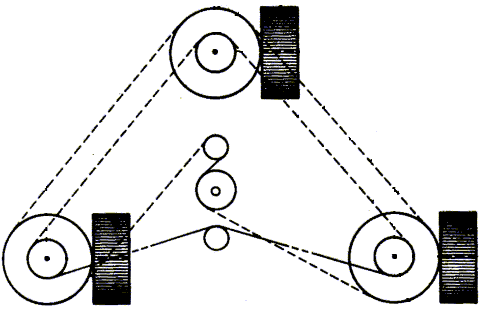
\includegraphics[width=3cm]{synchrodrive-simple}};


        \node[align=center, fill=hriSec3Comp!60,font=\footnotesize, text width=3cm, opacity=0.8,text opacity=1, draw,rectangle callout,anchor=pointer,callout relative pointer={(200:1)}] at (freewheel) {Empty: free wheel};

        \node[align=center, fill=hriSec3Comp!60,font=\footnotesize, text width=3cm, opacity=0.8,text opacity=1, draw,rectangle callout,anchor=pointer,callout relative pointer={(200:0.5)},right=1 of synchro] {Synchro drive aka omnidrive};

        \node[align=center, fill=hriSec3Comp!60,font=\footnotesize, text width=4cm, opacity=0.8,text opacity=1,draw,rectangle callout,anchor=pointer,callout relative pointer={(200:0.5)}] at (omni) {Omnidirectional drive};


    \end{tikzpicture}



\end{frame}

\begin{frame}{Different Arrangements of Wheels II}

Four wheels

    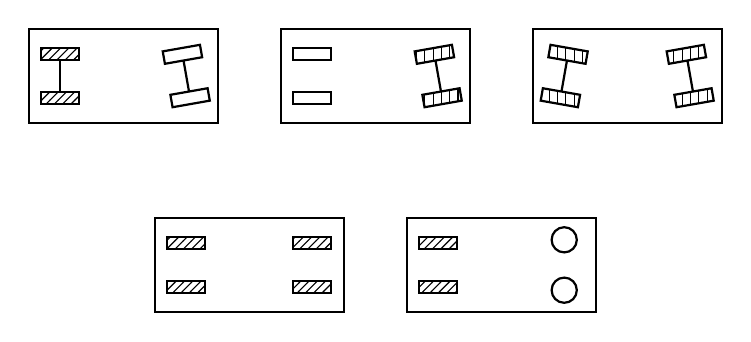
\begin{tikzpicture} 
        [>=latex,label/.style={align=center,font=\footnotesize},scale=0.8]

        \begin{scope}[shift={(0,0)}]
            \draw[thick] (0,0) rectangle (3,1.5);
            \draw[thick, pattern=north east lines] (0.2,0.3) rectangle +(0.6,0.2);
            \draw[thick, pattern=north east lines] (0.2,1.2) rectangle +(0.6,-0.2);
            \draw[thick] (0.5,0.5) -- (0.5,1);

            \begin{scope}[rotate around={10:(2.5,0.75)}, shift={(2.5,0.75)}]
                \draw[thick] (-0.3,0.25) rectangle +(0.6,0.2);
                \draw[thick] (-0.3,-0.25) rectangle +(0.6,-0.2);
                \draw[thick] (0,0.25) -- (0,-0.25);
            \end{scope}

        \end{scope}

        \begin{scope}[shift={(4,0)}]
            \draw[thick] (0,0) rectangle (3,1.5);
            \draw[thick] (0.2,0.3) rectangle +(0.6,0.2);
            \draw[thick] (0.2,1.2) rectangle +(0.6,-0.2);

            \begin{scope}[rotate around={10:(2.5,0.75)}, shift={(2.5,0.75)}]
                \draw[thick, pattern=vertical lines] (-0.3,0.25) rectangle +(0.6,0.2);
                \draw[thick, pattern=vertical lines] (-0.3,-0.25) rectangle +(0.6,-0.2);
                \draw[thick] (0,0.25) -- (0,-0.25);
            \end{scope}
        \end{scope}

        \begin{scope}[shift={(8,0)}]
            \draw[thick] (0,0) rectangle (3,1.5);
            \begin{scope}[rotate around={-10:(.5,0.75)}, shift={(.5,0.75)}]
                \draw[thick, pattern=vertical lines] (-0.3,0.25) rectangle +(0.6,0.2);
                \draw[thick, pattern=vertical lines] (-0.3,-0.25) rectangle +(0.6,-0.2);
                \draw[thick] (0,0.25) -- (0,-0.25);
            \end{scope}
            \begin{scope}[rotate around={10:(2.5,0.75)}, shift={(2.5,0.75)}]
                \draw[thick, pattern=vertical lines] (-0.3,0.25) rectangle +(0.6,0.2);
                \draw[thick, pattern=vertical lines] (-0.3,-0.25) rectangle +(0.6,-0.2);
                \draw[thick] (0,0.25) -- (0,-0.25);
            \end{scope}
        \end{scope}

        \begin{scope}[shift={(2,-3)}]
            \draw[thick] (0,0) rectangle (3,1.5);
            \draw[thick, pattern=north east lines] (0.2,0.3) rectangle +(0.6,0.2);
            \draw[thick, pattern=north east lines] (0.2,1.2) rectangle +(0.6,-0.2);
            \draw[thick, pattern=north east lines] (2.2,0.3) rectangle +(0.6,0.2);
            \draw[thick, pattern=north east lines] (2.2,1.2) rectangle +(0.6,-0.2);
        \end{scope}

        \begin{scope}[shift={(6,-3)}]
            \draw[thick] (0,0) rectangle (3,1.5);
            \draw[thick, pattern=north east lines] (0.2,0.3) rectangle +(0.6,0.2);
            \draw[thick, pattern=north east lines] (0.2,1.2) rectangle +(0.6,-0.2);
            \draw[thick] (2.5,0.35) circle[radius=0.2];
            \draw[thick] (2.5,1.15) circle[radius=0.2];
        \end{scope}

    \end{tikzpicture} 

Six wheels

    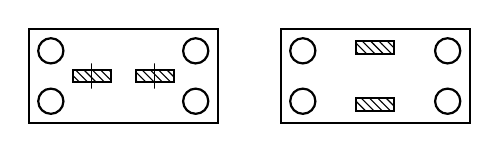
\begin{tikzpicture} 
        [>=latex,label/.style={align=center,font=\footnotesize},scale=0.8]


        \begin{scope}[shift={(2,0)}]
            \draw[thick] (0,0) rectangle (3,1.5);
            \draw[thick] (0.35,0.35) circle[radius=0.2];
            \draw[thick] (0.35,1.15) circle[radius=0.2];
            \draw[thick] (2.65,0.35) circle[radius=0.2];
            \draw[thick] (2.65,1.15) circle[radius=0.2];
            \draw (1,0.55) rectangle +(0,0.4);
            \draw[thick,pattern=north west lines] (0.7,0.65) rectangle +(0.6,0.2);
            \draw (2,0.55) rectangle +(0,0.4);
            \draw[thick,pattern=north west lines] (1.7,0.65) rectangle +(0.6,0.2);
        \end{scope}

        \begin{scope}[shift={(6,0)}]
            \draw[thick] (0,0) rectangle (3,1.5);
            \draw[thick] (0.35,0.35) circle[radius=0.2];
            \draw[thick] (0.35,1.15) circle[radius=0.2];
            \draw[thick] (2.65,0.35) circle[radius=0.2];
            \draw[thick] (2.65,1.15) circle[radius=0.2];
            \draw[thick,pattern=north west lines] (1.2,1.3) rectangle +(0.6,-0.2);
            \draw[thick,pattern=north west lines] (1.2,0.2) rectangle +(0.6,0.2);
        \end{scope}


    \end{tikzpicture} 



\end{frame}

\begin{frame}{Instantaneous centre of curvature (ICC)}

In order for all wheels of a vehicle to \textbf{roll} without
slipping, the axes of all wheels need to intersect in one point.

This point is called the ICC.

    \begin{center}
        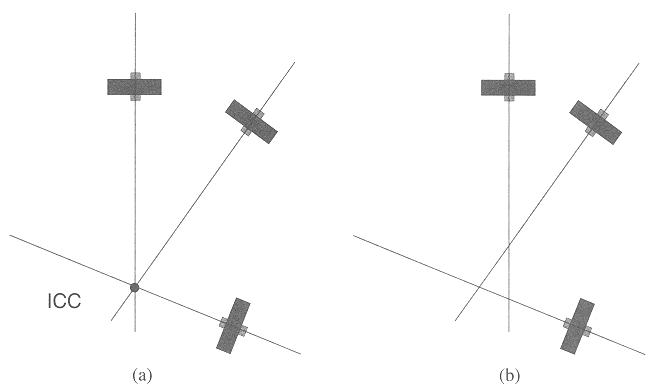
\includegraphics[width=0.7\linewidth]{icc}
    \end{center}
\end{frame}

\begin{frame}{Differential drive configuration}

    \begin{columns}
        \begin{column}{0.6\linewidth}

            Most used wheeled robot configuration

            \begin{itemize}
                \item Cheap (two motor on two drive wheels, one support wheel).
                \item Motors do driving and steering together.
                \item Excellent steering behaviour.
                \item Turn on the spot.
                \item However, relatively poor straight forward driving and cannot carry
                    heavy weights (the supporting wheels is critical here).
            \end{itemize}
        \end{column}
        \begin{column}{0.4\linewidth}

        \begin{center}
            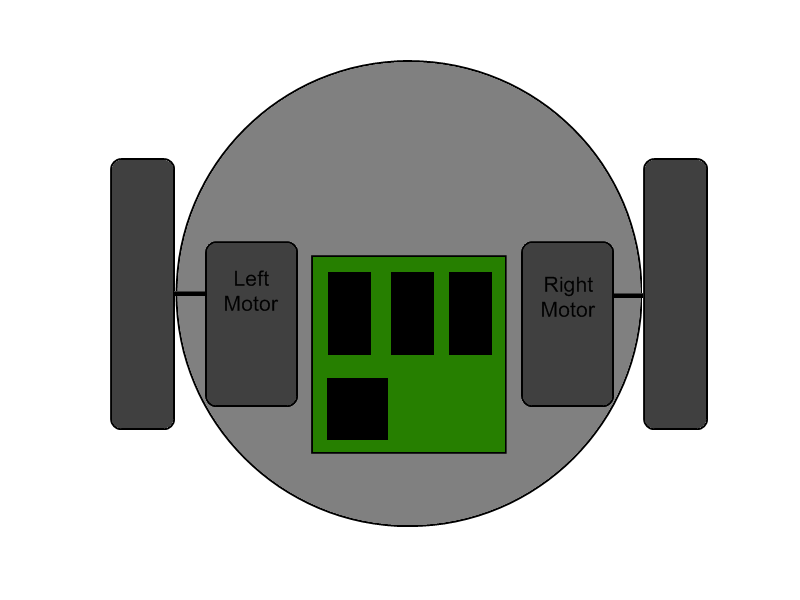
\includegraphics[width=0.8\linewidth]{differentialdrive}

            \source{cognitoware.com}{cognitoware}
        \end{center}
        \end{column}
    \end{columns}

\end{frame}

\begin{frame}{Some examples}

    \begin{columns}
        \begin{column}{0.5\linewidth}

            \begin{center}
                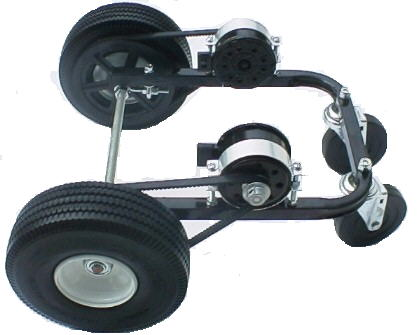
\includegraphics[width=0.7\linewidth]{differentialdrive_ex1}

                \source{www.kadtronix.com}{kadtronix}


                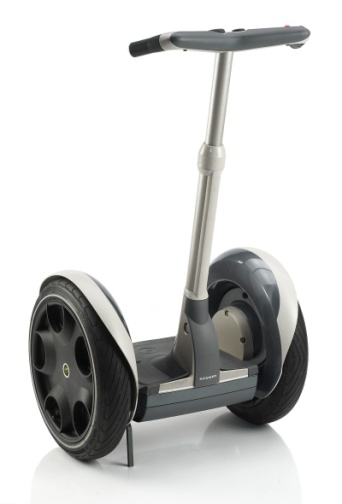
\includegraphics[width=0.4\linewidth]{differentialdrive_ex3}

                Segway
            \end{center}

        \end{column}
        \begin{column}{0.5\linewidth}
            \begin{center}
                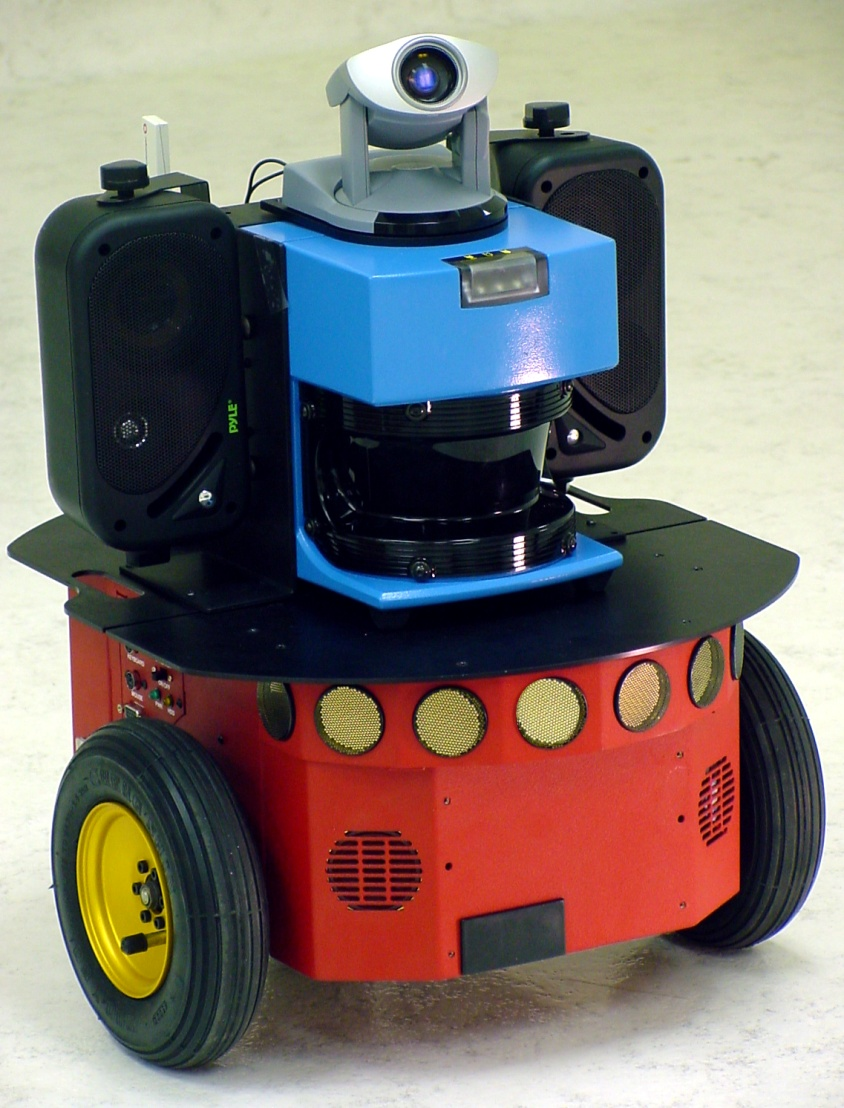
\includegraphics[width=0.7\linewidth]{differentialdrive_ex2}

                Pioneer
            \end{center}

        \end{column}
    \end{columns}
\end{frame}

\begin{frame}{Synchro Drive}

    \begin{columns}
        \begin{column}{0.6\linewidth}

            All wheels are actuated synchronously by one motor

            \begin{itemize}
                \item defines the speed of the vehicle
            \end{itemize}

            All wheels steered synchronously by a second motor

            \begin{itemize}
                \item sets the heading of the vehicle
            \end{itemize}

            The orientation in space of the robot frame will always remain the same

            \begin{itemize}
                \item It is therefore not possible to control the orientation of the robot
                    frame.
            \end{itemize}
        \end{column}
        \begin{column}{0.4\linewidth}

            \begin{center}
                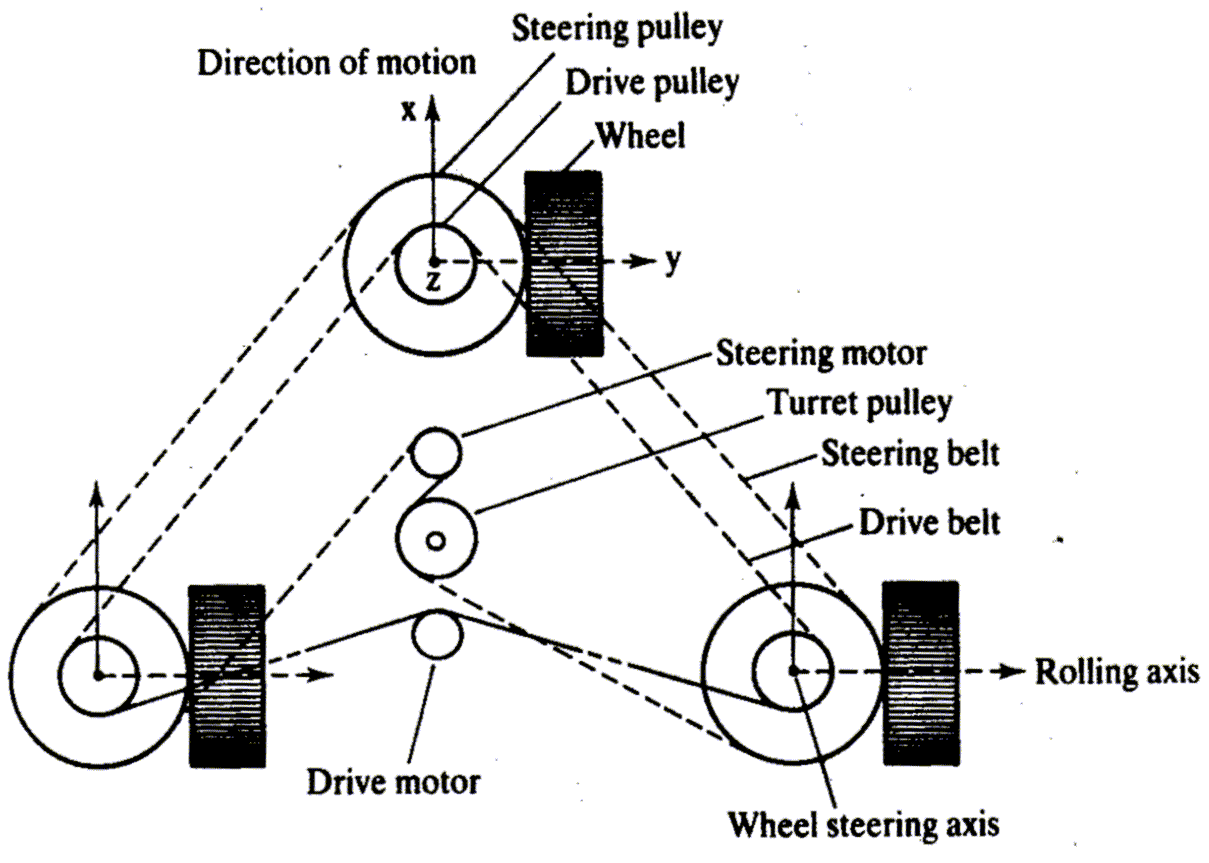
\includegraphics[width=0.8\linewidth]{synchrodrive}
            \end{center}
        \end{column}
    \end{columns}

\end{frame}

\begin{frame}{Synchro Drive}

\begin{itemize}
    \item Only for indoor robots.
    \item Very precise and excellent dead reckoning capabilities.
    \item Example: PR2 from Willow Garage, B12, B21 robots by Real World
  Interfaces, popular in the research labs.
\end{itemize}

    \begin{center}
        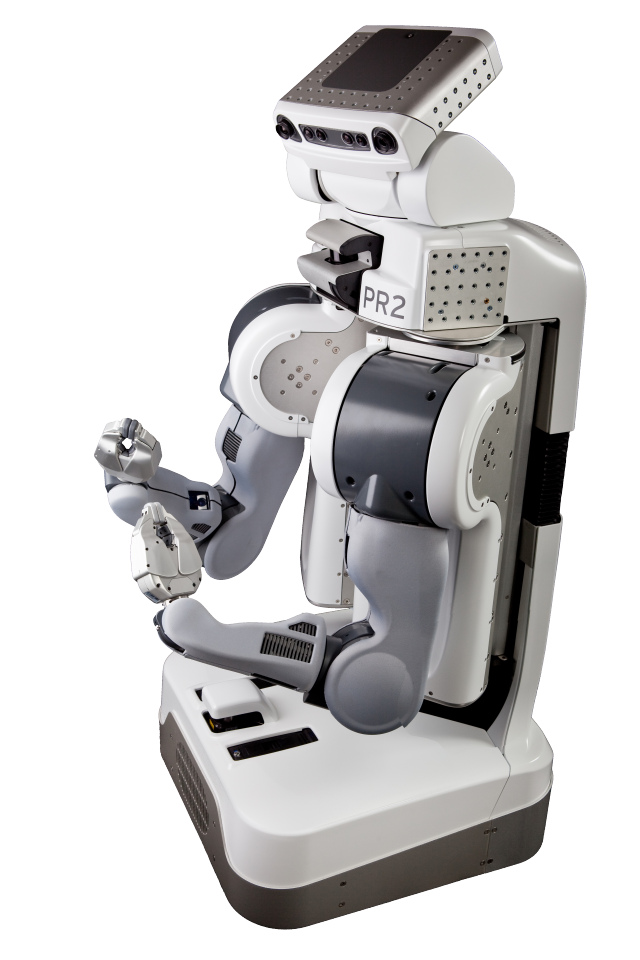
\includegraphics[height=0.4\paperheight]{pr2}
        \hspace{1em}
        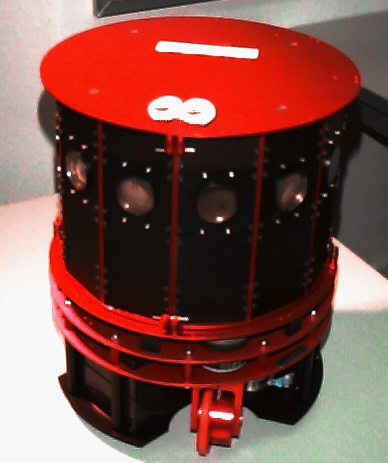
\includegraphics[height=0.4\paperheight]{synchrodrive_ex1}
        \hspace{1em}
        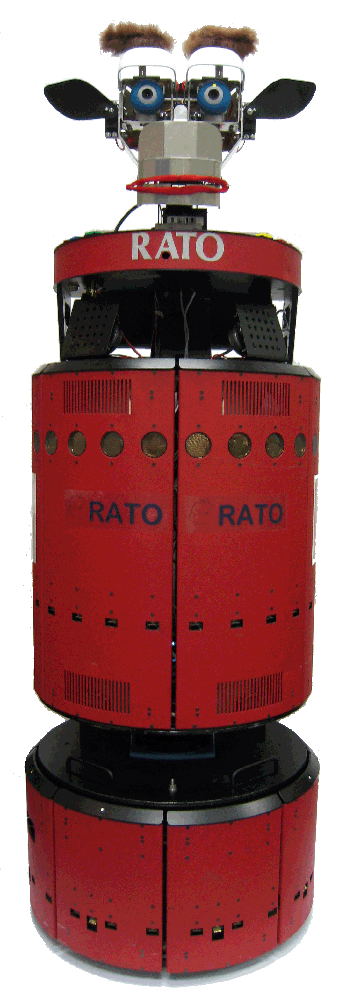
\includegraphics[height=0.4\paperheight]{b21}
    \end{center}

\end{frame}

\begin{frame}{Stepping / Walking with Wheels}

\begin{itemize}
    \item SpaceCat, and micro-rover for Mars, developed by Mecanex Sa and EPFL
  for the European Space Agency (ESA)
\end{itemize}

    \begin{center}
        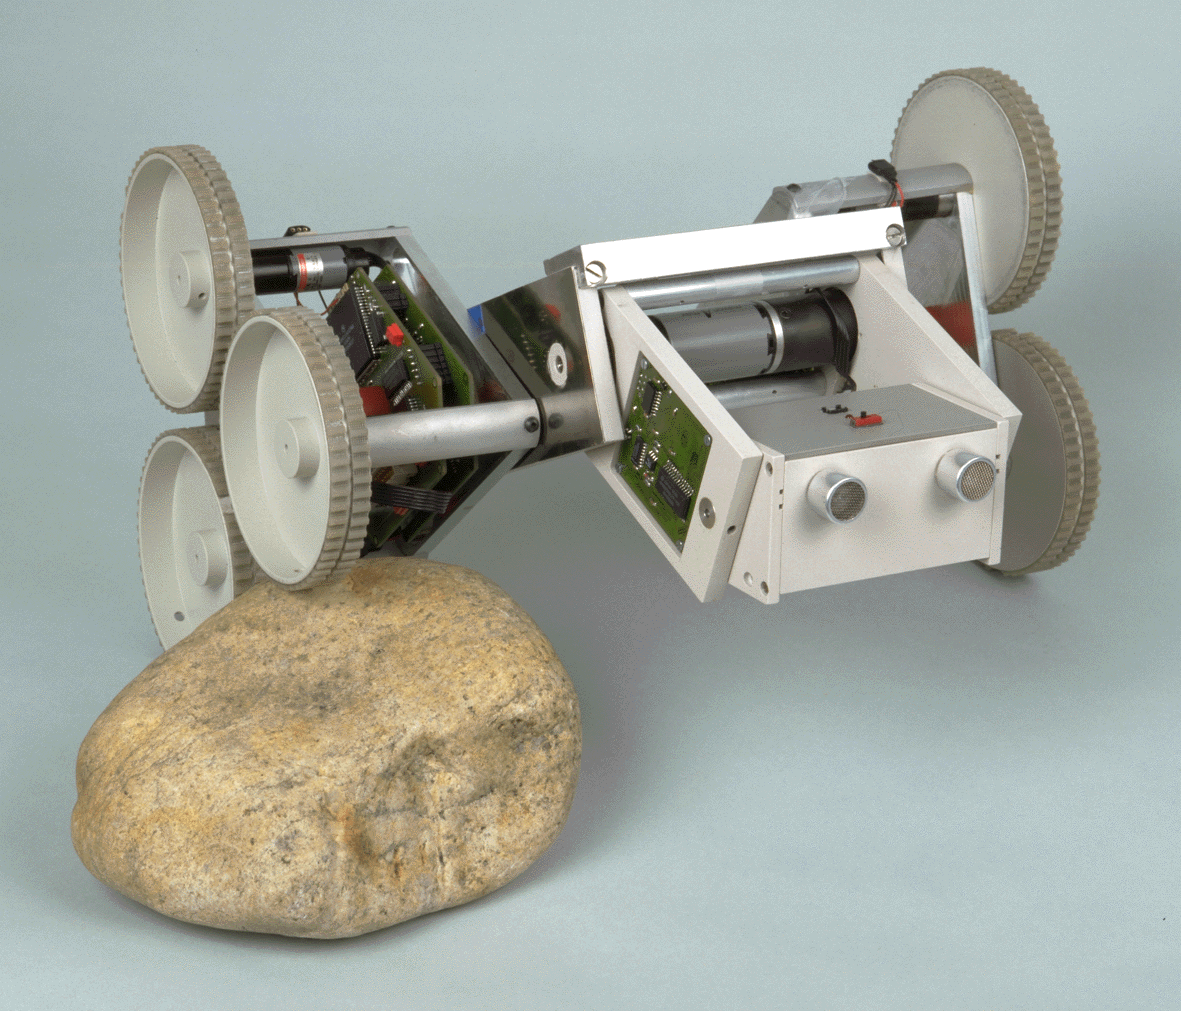
\includegraphics[width=0.4\linewidth]{walkingwheels_ex1}
        
\includegraphics[width=0.4\linewidth]{walkingwheels_ex2}
    \end{center}
\end{frame}

\begin{frame}{Shrimp, a Mobile Robot with Excellent Climbing Abilities}

Objective

\begin{itemize}
    \item Passive locomotion concept for rough terrain
\end{itemize}

Results: The Shrimp

6 wheels

\begin{itemize}
    \item one fixed wheel in the rear
    \item two boogies on each side
    \item one front wheel with spring suspension
\end{itemize}

robot measures around 60 cm in length and 20 cm in height

highly stable in rough terrain

overcomes obstacles up to 2 times its wheel diameter

    \begin{center}
        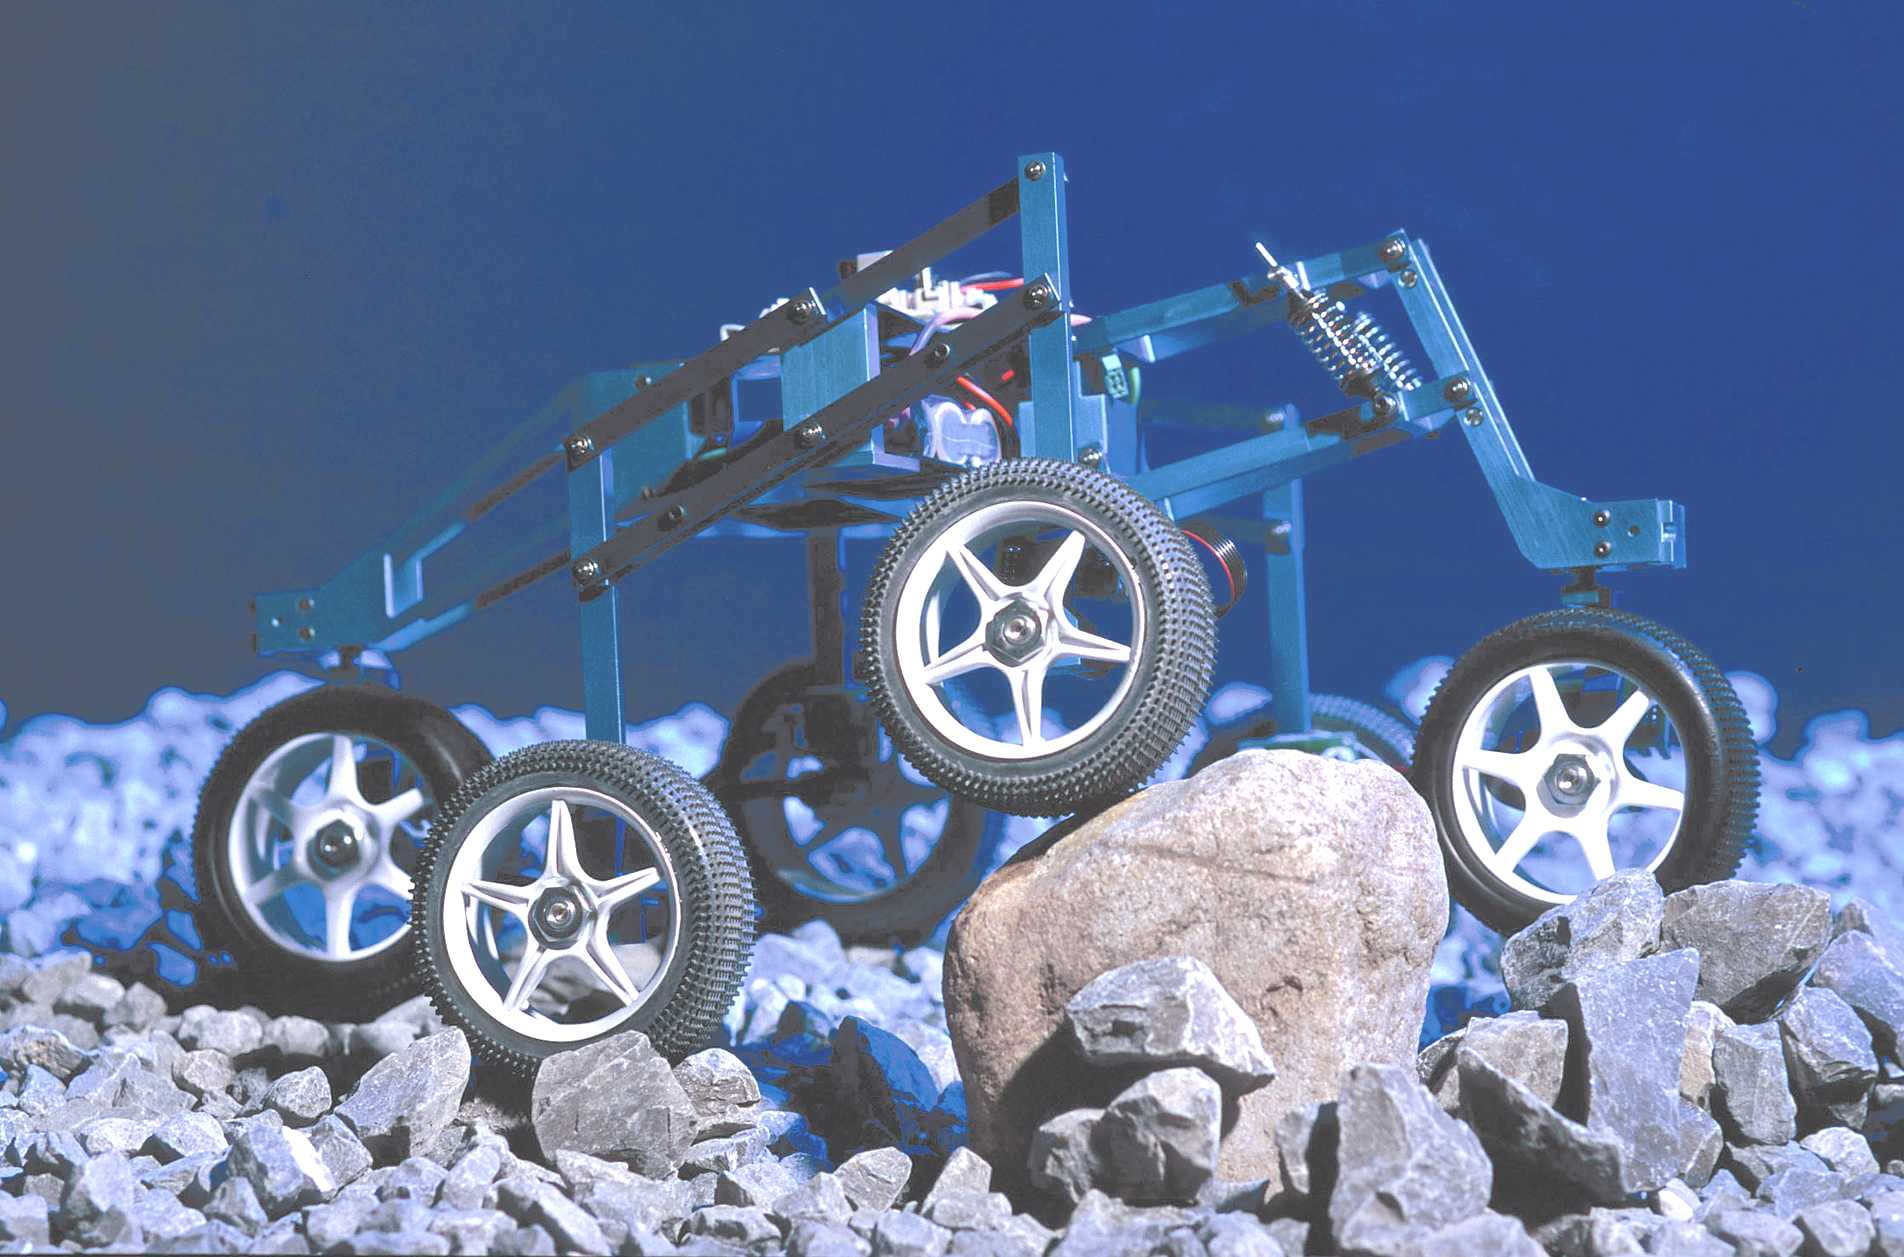
\includegraphics[width=0.8\linewidth]{shrimp}
    \end{center}
\end{frame}

\begin{frame}{Shrimp}

\begin{center}
    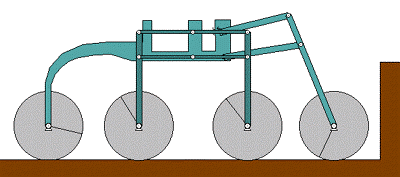
\includegraphics[width=0.2\linewidth]{shrimp1}
    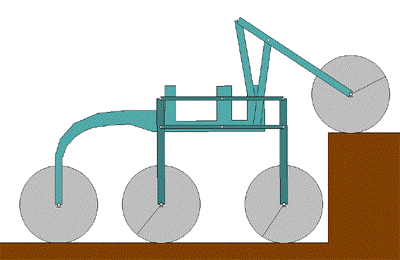
\includegraphics[width=0.2\linewidth]{shrimp2}
    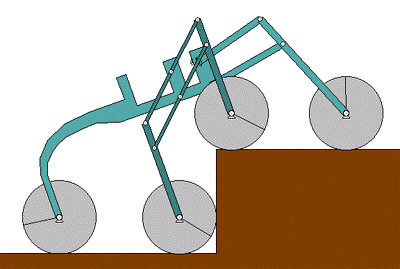
\includegraphics[width=0.2\linewidth]{shrimp3}
    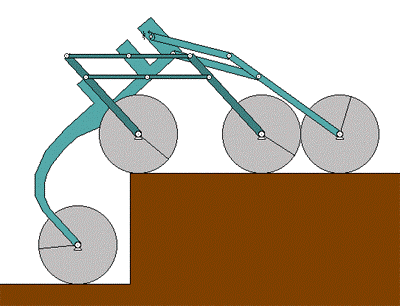
\includegraphics[width=0.2\linewidth]{shrimp4}
\end{center}

    \begin{center}
        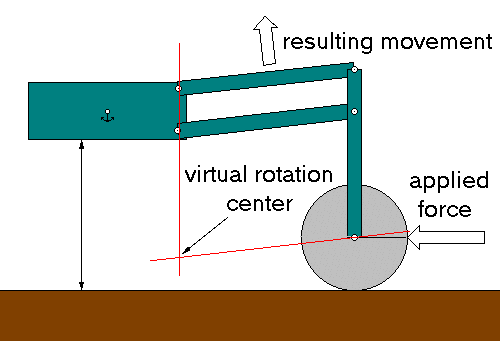
\includegraphics[width=0.4\linewidth]{shrimp_leg}
    \end{center}

\end{frame}

\begin{frame}{Tracked drive}

\begin{itemize}
    \item Same principle as differential drive, but instead of wheels the robot
  has tracks.
    \item Good grip, low slippage. Excellent for rough terrain.
    \item Very unpredictable rotation.
\end{itemize}

    \begin{center}
        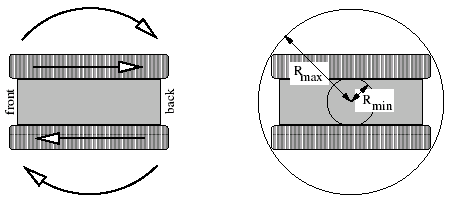
\includegraphics[width=0.8\linewidth]{tracked_drive}
    \end{center}
\end{frame}

\begin{frame}{Ackerman drive}

    \only<1>{
        Four wheels, just as a car.

    Front wheels for steering.

    When turning, all wheels turn at different speeds.

    \begin{itemize}
        \item Is resolved for the back wheels by a differential gear.
    \end{itemize}

    \begin{center}
        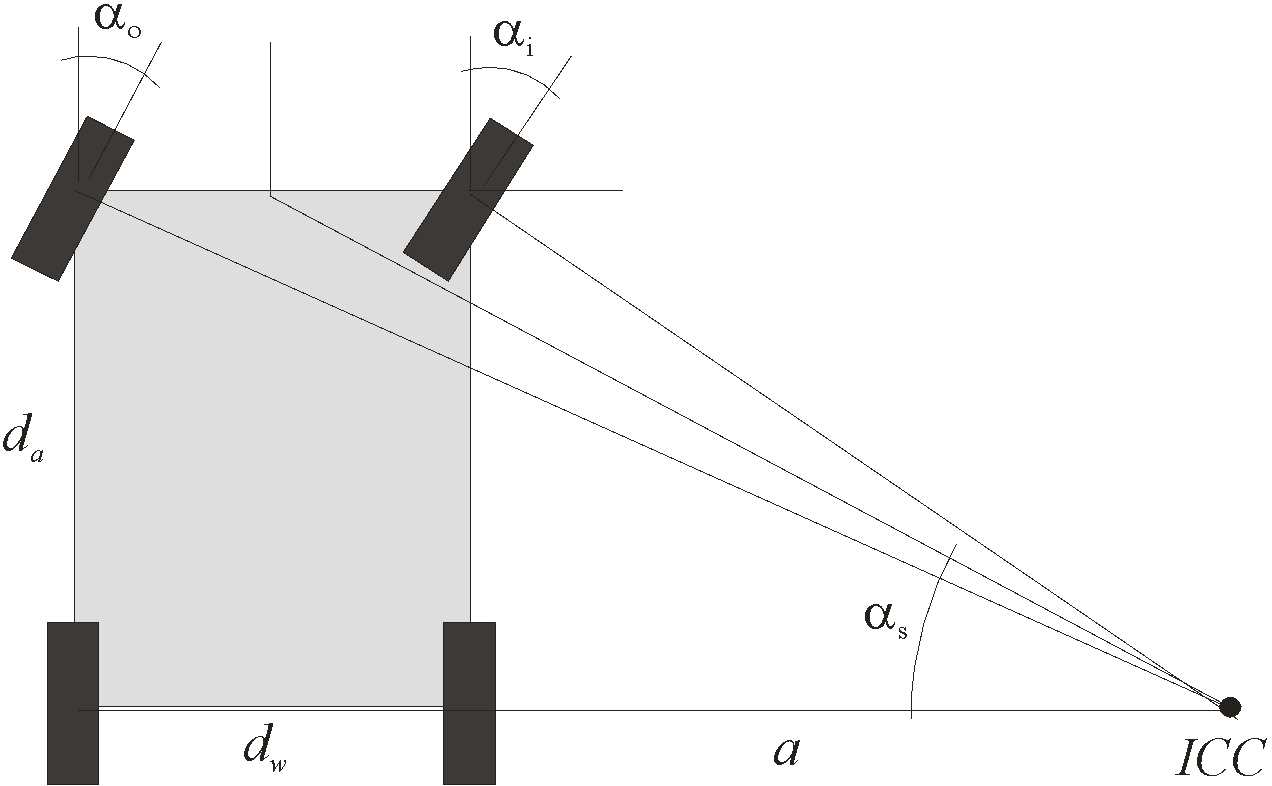
\includegraphics[width=0.6\linewidth]{ackerman_drive}
    \end{center}
}
    \only<2>{

        \begin{itemize}
            \item Front wheels need different steering angle, to avoid slippage. Given
                by\ldots{}
        \end{itemize}

    \begin{align*}
        a &= \frac{d_a}{tan(a_i)} - d_w \\
        a_i &= tan^{-1}(\frac{d_a}{a}) \\
        tan(a_s) &= \frac{d_a}{a + \frac{d_w}{2}}
    \end{align*}
}
\end{frame}

\begin{frame}{Balldrive}
    \begin{center}
        \includegraphics<1>[width=0.9\linewidth]{balldrive-cellulo}
        \includegraphics<2>[width=0.9\linewidth]{magnetic_ball_drive}
        \includegraphics<3>[width=0.9\linewidth]{balldrive-cellulo-model}

        \source{http://ayberkozgur.com/_media/publications:balldrive.pdf}{\"Ozg\"ur et al., Permanent Magnet-Assisted Omnidirectional Ball Drive}
    \end{center}
\end{frame}

\videoframe[0.56]{figs/part4/cellulo.mp4?start=3}

\begin{frame}{Balldrive vs. omniwheels}
    \begin{columns}
        \begin{column}{0.4\linewidth}
            \begin{center}
                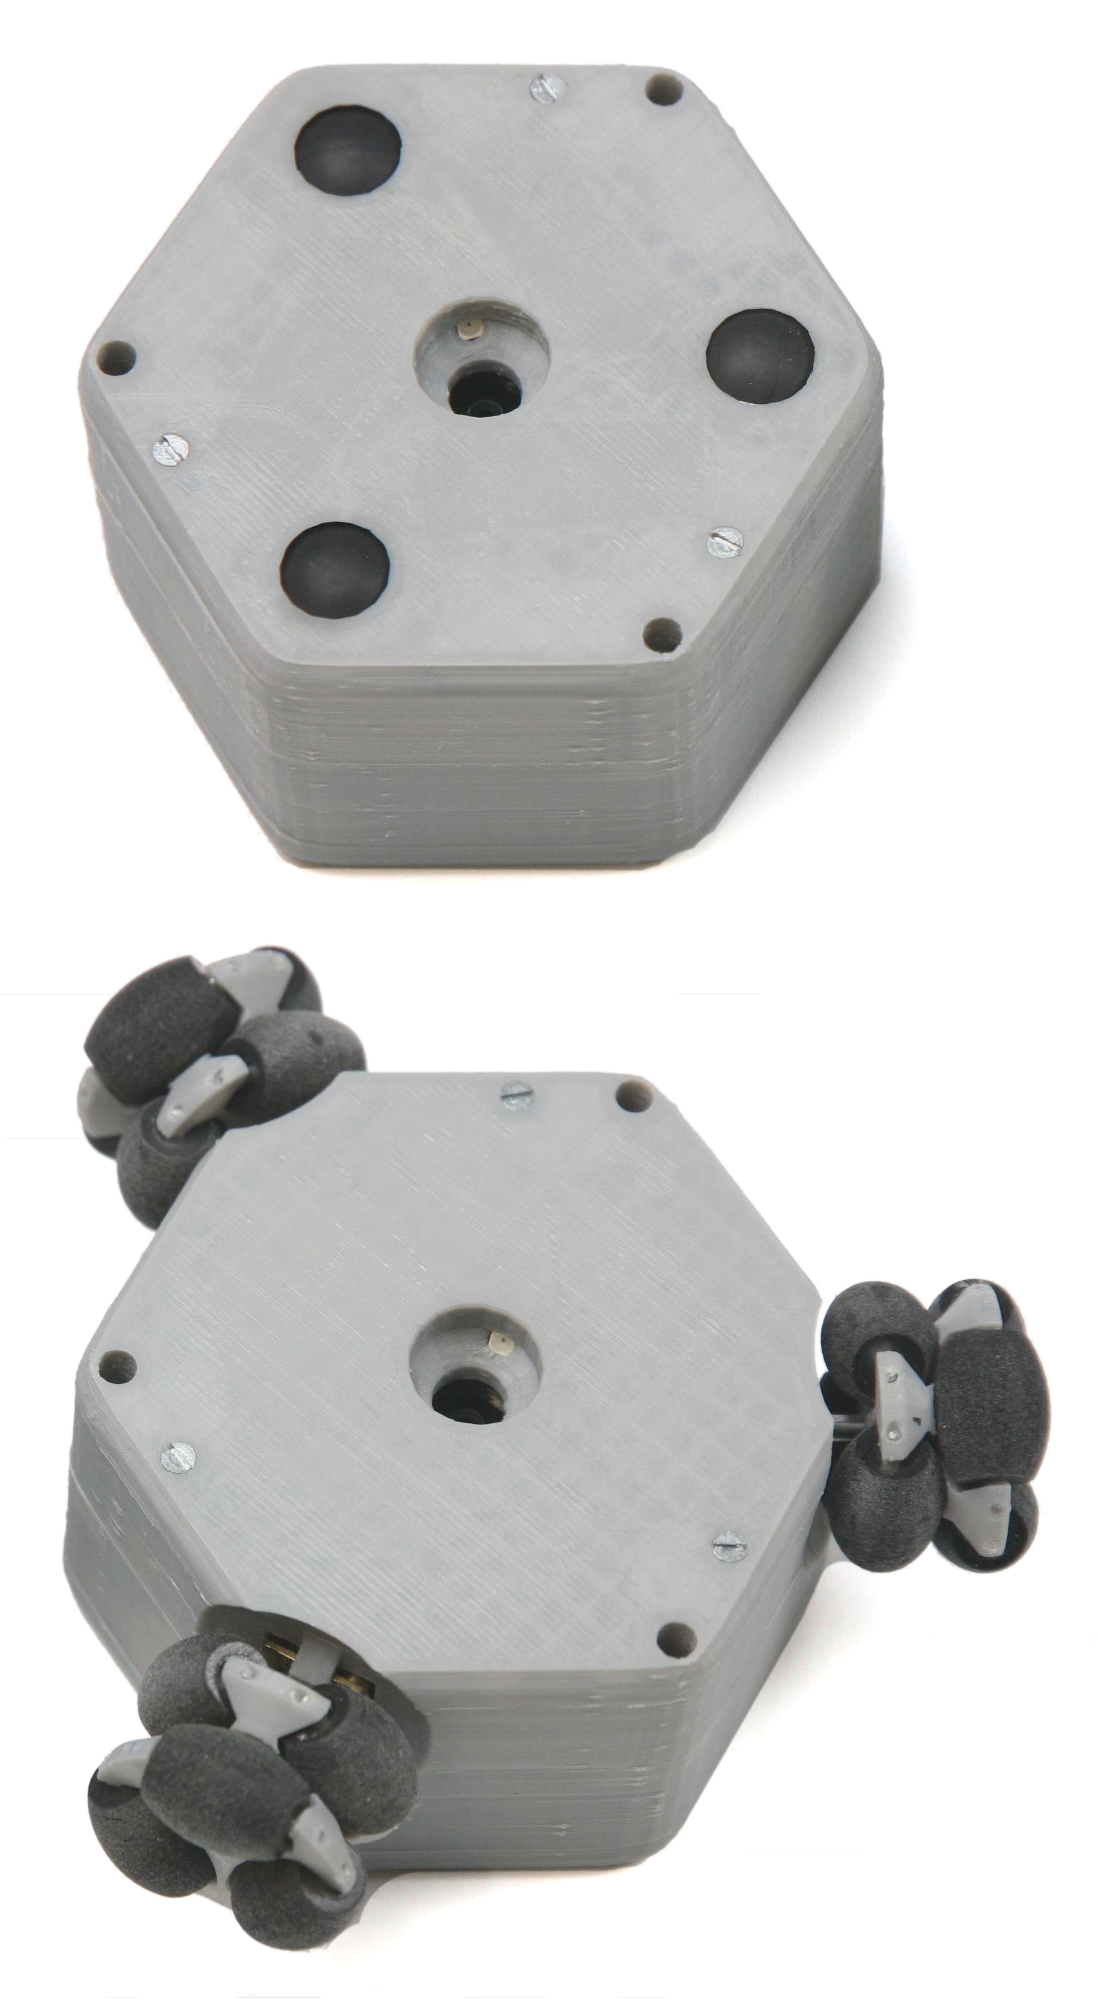
\includegraphics[width=0.8\linewidth]{balldrive-omniwheel}
            \end{center}
        \end{column}
        \begin{column}{0.6\linewidth}
            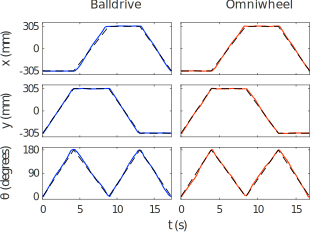
\includegraphics[width=\linewidth]{balldrive-vs-omniwheel}
        \end{column}
    \end{columns}

    \begin{center}

        \source{http://ayberkozgur.com/_media/publications:balldrive.pdf}{\"Ozg\"ur et al., Permanent Magnet-Assisted Omnidirectional Ball Drive}
    \end{center}

\end{frame}

%%%%%%%%%%%%%%%%%%%%%%%%%%%%%%%%%%%%%%%%%%%%%%%%%%%%%%%%%%%%%%%%%%%%%%%%%%
%%%%%%%%%%%%%%%%%%%%%%%%%%%%%%%%%%%%%%%%%%%%%%%%%%%%%%%%%%%%%%%%%%%%%%%%%%
%%%%%%%%%%%%%%%%%%%%%%%%%%%%%%%%%%%%%%%%%%%%%%%%%%%%%%%%%%%%%%%%%%%%%%%%%%

\section{Kinematics}

\begin{frame}{Kinematics vs dynamics}

\href{http://en.wikipedia.org/wiki/Kinematics}{Kinematics} describes the
motion of objects or systems (combination of objects), but does not take
forces into account. No mass, friction, gravity, momentum, \ldots{}

\href{http://en.wikipedia.org/wiki/Analytical_dynamics}{Dynamics} take
forces into account.

\begin{itemize}
    \item \href{http://www.youtube.com/watch?v=kEed8DVO21I}{Weightlifting
  robot}, using dynamics to overcome the weight limitation.
\end{itemize}

Kinematics is simpler than dynamics. This module only considers
kinematics.

\end{frame}

\begin{frame}{Mobile robot kinematics}

    \begin{columns}
        \begin{column}{0.6\linewidth}
            Aim: description of mechanical behavior of the robot for \emph{control}

            Similar to robot manipulator kinematics

            However, a mobile robot can move unbounded with respect to its
            environment

            \begin{itemize}
                \item There is no direct way to measure the robot's position
                \item Position must be integrated over time
                \item Leads to inaccuracies of the position (motion) estimate
                    $\rightarrow$ a major challenge in mobile robotics
            \end{itemize}

        \end{column}
        \begin{column}{0.4\linewidth}
            \begin{center}
                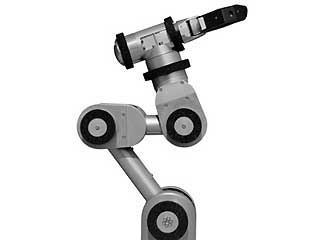
\includegraphics[width=\linewidth]{kinematics_ex1}
            \end{center}
        \end{column}
    \end{columns}

\end{frame}

\begin{frame}{Forward and inverse kinematics}


    \only<1>{
        \textbf{Forward kinematics}

    Calculate the position, orientation and speed of robot as a function of
    its wheel angles and speeds.

    \begin{itemize}
        \item Example 1: inverse kinematics in a robot arm tells you the position of
            the robot hand in function of the joint angles.
        \item Example 2: when you know the speed of the left and right wheel of a
            differential drive robot, you know the velocity of the robot body.
    \end{itemize}

}
    \only<2>{
        \textbf{Inverse kinematics}

    Calculate the wheel angles and speeds to achieve a certain robot speed
    or robot position and orientation.

    \begin{itemize}
        \item Example 1: if the robot hand needs to be in position (x,y,z), what
            joint angles should the robot arm have?
        \item Example 2: if the you want the robot to drive at v m/s and rotate at θ
            rad/s, what should the wheels do?
    \end{itemize}

    \alert{Inverse Kinematics is harder because there are most often several
    (sometimes infinite) solutions to the problem.}

    \begin{itemize}
        \item For example: you can reach a point with a robot hand with any number
            of joint angles.
    \end{itemize}
}
\end{frame}

\begin{frame}{A kinematics model}

    Goal: establish the robot speed $\dot\xi = \begin{bmatrix} \dot{x} & \dot{y}
    & \dot{\theta}\end{bmatrix}^T$  as a function of the wheel speeds
        $\dot\varphi_i$, steering
    angles $\beta_i$, steering speeds $\dot\beta_i$ and the geometric parameters of the robot
    (\emph{configuration coordinates}).

        \begin{columns}
            \begin{column}{0.7\linewidth}
                Forward kinematics:

                \[
                    \dot\xi = \colvec{\dot{x} \\ \dot{y} \\ \dot{\theta} } = f(\dot\varphi_1,\ldots,\dot\varphi_n,\beta_1,\ldots,\beta_m,\dot\beta_1,\ldots,\dot\beta_m)
                \]

            \end{column}
            \begin{column}{0.3\linewidth}
                \begin{center}
                    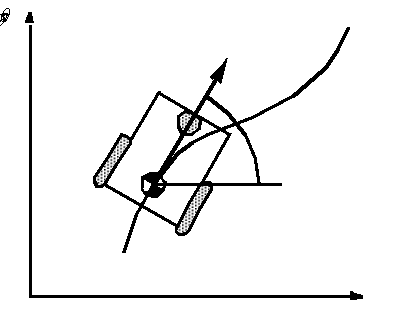
\includegraphics[width=\linewidth]{kinematic_model}
                \end{center}

            \end{column}
        \end{columns}


        \pause

    Inverse kinematics:

    $
        \colvec{\dot\varphi_1 & \ldots & \dot\varphi_n& \beta_1 & \ldots &
        \beta_m & \dot\beta_1 & \ldots & \dot\beta_m}^T = f(\dot{x},
        \dot{y},\dot\theta)
    $

Note that  $\colvec{x \\ y \\ \theta } =
        f(\varphi_1,\ldots,\varphi_n,\beta_1,\ldots,\beta_m)$ does not make sense. Why?

        %\href{http://en.wikipedia.org/wiki/Transpose}{Transpose} of a matrix A
        %is written as AT : write rows of A as columns.
        %
        %A dot above a variable refers to its derivative in time: the speed at
        %which it changes. Also written as

\end{frame}

\begin{frame}{Representing robot position}

Representing the robot within an arbitrary initial frame

    \begin{columns}
        \begin{column}{0.6\linewidth}
\begin{itemize}
    \item Initial frame: ${X_I, Y_I}$
    \item Robot frame: ${X_R, Y_R}$
    \item Robot position: $\xi_I = \colvec{x & y & \theta}^T$
\end{itemize}

            \vspace{1em}

Mapping between the two frames:

    \begin{align*}
        \dot\xi_R &= R(\theta)\cdot \dot\xi_I = R(\theta)\cdot \colvec{\dot{x} \\ \dot{y} \\ \dot\theta} \\ 
        R(\theta) &= \begin{bmatrix} cos\theta & sin\theta & 0 \\
                                    -sin\theta & cos\theta & 0 \\
                                             0 &         0 & 1 \end{bmatrix}
    \end{align*}

            
        \end{column}
        \begin{column}{0.4\linewidth}

    \begin{center}
        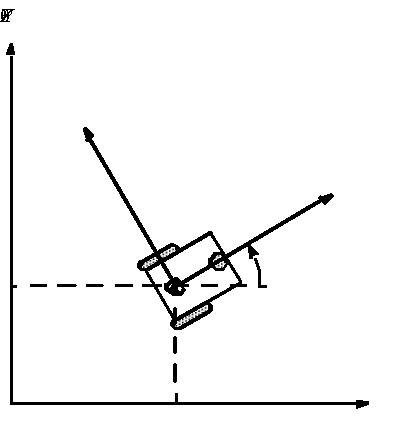
\includegraphics[width=0.9\linewidth]{robot_position}
    \end{center}
        \end{column}
    \end{columns}



\end{frame}

\begin{frame}{Example: robot aligned with $Y_I$}
    \begin{columns}
        \begin{column}{0.6\linewidth}

    \begin{align*}
        R(\theta) &= \begin{bmatrix} cos\theta & sin\theta & 0 \\
                                    -sin\theta & cos\theta & 0 \\
                                             0 &         0 & 1 \end{bmatrix}
    \end{align*}

            
        \end{column}
        \begin{column}{0.4\linewidth}

    \begin{center}
        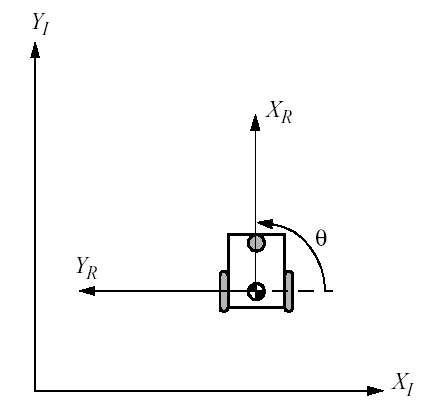
\includegraphics[width=0.9\linewidth]{robot_position_simple}
    \end{center}
        \end{column}
    \end{columns}


    \begin{align*}
        \dot\xi_R &= R(\frac{\pi}{2})\cdot \dot\xi_I = \begin{bmatrix} 0 & 1 & 0 \\
                                                                      -1 & 0 & 0 \\
                                                                       0 & 0 & 1 \end{bmatrix} \cdot \colvec{\dot{x} \\ \dot{y} \\ \dot\theta} =  \colvec{\dot{y} \\ -\dot{x} \\ \dot\theta} 
    \end{align*}



\end{frame}

\begin{frame}{Kinematics of a wheeled robot}

The kinematics of a robot can be understood by looking at the kinematics
of the individual wheels.

But we need to assume some stringent constraints

\begin{itemize}
    \item Movement on a horizontal plane
    \item Point contact of the wheels
    \item Wheels not deformable
    \item Pure rolling
    \item No slipping, skidding or sliding
    \item No friction for rotation around contact point
    \item Steering axes orthogonal to the surface
    \item Wheels connected by rigid frame (chassis)
\end{itemize}

If these constraints are not met, our calculations will be off.

\end{frame}

\section{Differential drive}

\begin{frame}{Forward kinematics of differential drive (1)}

    \begin{columns}
        \begin{column}{0.5\linewidth}


            Differential drive robot

            \begin{itemize}
                \item Two wheels with radius $r$
                \item Distance between wheels is $2\cdot l$
                \item Orientation wrt inertial basis is $\theta$
                \item Turning speed of wheels is $\dot\varphi_1, \dot\varphi_2$
            \end{itemize}

        \end{column}
        \begin{column}{0.5\linewidth}


            \resizebox{0.8\linewidth}{!}{
                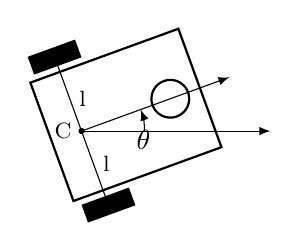
\begin{tikzpicture} 
                    [>=latex,label/.style={align=center,font=\footnotesize},scale=0.8]


                    \begin{scope}[rotate=20, shift={(2,0)}]
                        \coordinate (O) at (0,0) node[label, left] {C};
                        \fill[thick] (O) circle[radius=0.05];
                        \draw (O) -- (0,1.1) node[label,midway,right] {l};
                        \draw (O) -- (0,-1.1) node[label,midway,right] {l};
                        \draw[thick] (-0.5,-1) rectangle (2,1);
                        \draw[thick] (1.5,0) circle[radius=0.3];

                        \fill ($(0, 1.1) - (0.4,0)$) rectangle +(0.8,0.3);
                        \fill ($(0, -1.1) - (0.4,0)$) rectangle +(0.8,-0.3);

                        \draw[->] (O) -- +(2.5,0);
                        \draw[<-] (O) + (1,0) arc [start angle=0, end angle=-20, radius=1] node[midway,below] {$\theta$};
                    \end{scope}
                    \draw[->] (O) -- +(3,0);

                \end{tikzpicture}
            }

        \end{column}
    \end{columns}

    Robot's overall speed in global reference frame:

    \[
        \dot\xi_I = \colvec{\dot{x} \\ \dot{y} \\ \dot\theta} = f(l, r, \theta,
        \dot\varphi_1, \dot\varphi_2)
        \]

\end{frame}

\begin{frame}{Forward kinematics of differential drive (2)}

    The speed of a wheel over ground is

    \begin{columns}
        \begin{column}{0.5\linewidth}
            \resizebox{0.6\linewidth}{!}{%
                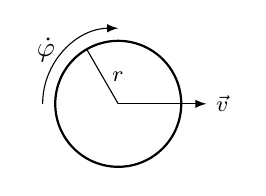
\begin{tikzpicture} 
                    [>=latex,label/.style={align=center,font=\footnotesize},scale=0.8]


                \draw[thick] (0,0) circle[radius=1];


                \draw[->] (-1.2,0) arc [start angle=180, end angle=90, radius=1.2] node[midway,left] {$\dot\varphi$};

                    \draw (0,0) -- +(120:1) node[label, midway,right] {$r$};
                    \draw[->] (0,0) -- +(0:1.4) node[label,right] {$\vec{v}$};

                \end{tikzpicture}
            }

        \end{column}
        \begin{column}{0.5\linewidth}
            \[
                \dot\varphi [rad/s]\cdot r [m] = v [m/s]
            \]
        \end{column}
    \end{columns}
    Consider one wheel turning, the other wheel stationary.
    \vspace{1em}

    \begin{columns}
        \begin{column}{0.5\linewidth}
The robot will pivot around the other wheel and the instantaneous
            contribution of the rotating wheel will be that point $p$ has a
            speed $v_p$.

            \[
                v_p = \frac{1}{2}\cdot v_1 = \frac{1}{2}\cdot \dot\varphi_1\cdot r
                \]

        \end{column}
        \begin{column}{0.5\linewidth}
            \resizebox{0.6\linewidth}{!}{%
                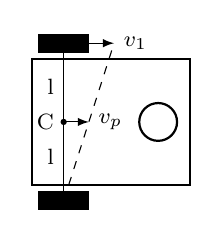
\begin{tikzpicture} 
                    [>=latex,label/.style={align=center,font=\footnotesize},scale=0.8]


                        \coordinate (O) at (0,0) node[label, left] {C};
                        \fill[thick] (O) circle[radius=0.05];
                        \draw (O) -- (0,1.1) node[label,midway,left] {l};
                        \draw (O) -- (0,-1.1) node[label,midway,left] {l};
                        \draw[thick] (-0.5,-1) rectangle (2,1);
                        \draw[thick] (1.5,0) circle[radius=0.3];

                        \fill ($(0, 1.1) - (0.4,0)$) rectangle +(0.8,0.3);
                        \fill ($(0, -1.1) - (0.4,0)$) rectangle +(0.8,-0.3);

                        \coordinate (wheel1) at (0,1.25);
                        \coordinate (wheel2) at (0,-1.25);
                        \draw[->] (wheel1) -- +(0.8,0) node[label,right] {$v_1$};
                        \draw[dashed] (wheel2) -- ($(wheel1) +(0.8,0)$);
                        \draw[->] (O) -- +(0.4,0) node[label,right] {$v_p$};

                \end{tikzpicture}
            }

        \end{column}
    \end{columns}

\end{frame}

\begin{frame}{Forward kinematics of differential drive (3)}

    The contribution of both wheels can be added together. So, when both
    wheel spin, the robot's mid point moves at

    \[
    v_p = \frac{1}{2}\cdot \dot\varphi_1\cdot r + \frac{1}{2}\cdot \dot\varphi_2\cdot r
    \]


            \begin{itemize}
                \item In particular, if wheel 1 has speed $\dot\varphi_1 = a$ and wheel 2 $\dot\varphi_2 = -a$ then the robot will turn
                    on the spot and have no translational speed: $v_p = 0$.
            \end{itemize}

    \pause

    The speed in the robot reference frame is:

    \begin{align*}
        \dot{x}_R &= v_p \\
        \dot{y}_R &= 0\bubblemark{nosideways}
    \end{align*}

    \bubble<1>{nosideways}{The robot cannot move sideways in a differential drive configuration}

\end{frame}

\begin{frame}{Forward kinematics of differential drive (4)}

    The rotational component $\dot\theta_R$ of $\dot\xi_R$ can be computed by adding the instantaneous
contribution of each wheel to the robots rotational velocity.

    \begin{columns}
        \begin{column}{0.5\linewidth}
            \centering
            \resizebox{0.3\linewidth}{!}{%
                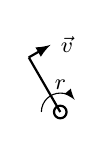
\begin{tikzpicture} 
                    [>=latex,label/.style={align=center,font=\footnotesize},scale=0.8]


                \draw[thick] (0,0) circle[radius=0.1];


                \draw[->] (-0.3,0) arc [start angle=180, end angle=40, radius=0.3];

                    \draw[thick] (0,0) -- +(120:1) node[label, midway,right] {$r$};
                    \draw[thick, ->] (120:1) -- +(30:.4) node[label,right] {$\vec{v}$};

                \end{tikzpicture}
            }

        \end{column}
        \begin{column}{0.5\linewidth}
            \[
                \omega [rad/s] = \frac{v [m/s]}{l [m]}
            \]
        \end{column}
    \end{columns}


For the left wheel and for the right wheel:
\[
    \omega_1 = \frac{\dot\varphi_1\cdot r}{2l};\qquad \omega_2 = -\frac{\dot\varphi_2\cdot r}{2l};
\]

Rotational velocity of robot after adding these two:

\[
    \dot\theta = \frac{r}{2l}\cdot (\dot\varphi_1 - \dot\varphi_2)
\]

\end{frame}

\begin{frame}{Forward kinematics of differential drive (5)}

Written in matrix form this is:

\[
    \dot\xi_R = \colvec{\dot{x} \\ \dot{y} \\ \dot\theta} = \colvec{r\cdot (\dot\varphi_1 + \dot\varphi_2) \\ 0 \\ \frac{r}{2l}\cdot (\dot\varphi_1 - \dot\varphi_2)}
\]


This can be remapped to the initial frame by:

\[
    \dot\xi_I = R(\theta)^{-1}\cdot \dot\xi_R
\]

\end{frame}

\begin{frame}{Practical approach}

    \only<1>{
Sampling interval $I$ for wheel encoders. Encoders report wheel
increment $N_L$ and $N_R$.

Assume that:
    \[
        c_m = \frac{2\pi r}{n\cdot C_e}
        \]

\begin{itemize}
    \item $r$ = wheel radius.
    \item $C_e$ = encoder resolution (in pulses per revolution).
    \item $n$ = gear ratio between motor and wheel.
    \item $c_m$ = conversion factor from encoder ticks to wheel
  displacement.
\end{itemize}
}
    \only<2>{

Incremental travel distance at time $i$ for left and right wheel is:

\begin{align*}
    \Delta U_{L,i} &= c_m\cdot N_{L,i} \\
    \Delta U_{R,i} &= c_m\cdot N_{R,i}
\end{align*}

Incremental linear displacement for robot's centerpoint $C$ is:

\[
        \Delta U_{i} = \frac{\Delta U_{L,i} + \Delta U_{R,i}}{2}
\]
}
    \only<3>{

Incremental change of orientation is
        
        
\[
        \Delta \theta_{i} = \frac{\Delta U_{L,i} - \Delta U_{R,i}}{b}
\]

        
        with $b = 2l$ the wheelbase, measured between the contact points of the wheels with the ground.

    The robots new state is:

\begin{align*}
    \theta_i &= \theta_{i-1} + \Delta\theta_i \\
    x_i &= x_{i-1} + \Delta U_i\cdot cos(\theta_i) \\
    y_i &= y_{i-1} + \Delta U_i\cdot sin(\theta_i) 
\end{align*}

}

    \only<4>{
        \begin{columns}
            \begin{column}{0.5\linewidth}
    Rotation radius $R$ is:

\begin{align*}
    \omega &= \frac{v_L}{R - l} = \frac{v_R}{R + l} \\
    \Rightarrow R &= l\cdot \frac{\Delta U_R + \Delta U_L}{\Delta U_R - \Delta U_L}
\end{align*}

            \end{column}
            \begin{column}{0.5\linewidth}
            \centering
            \resizebox{0.8\linewidth}{!}{%
                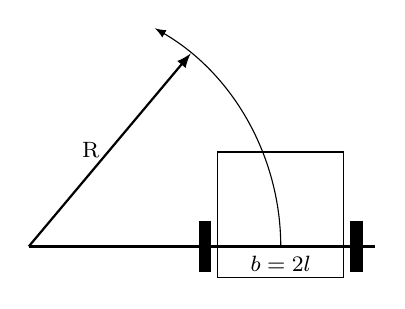
\begin{tikzpicture} 
                    [>=latex,label/.style={align=center,font=\footnotesize},scale=0.8]


                    \draw[thick] (0,0) -- (0:5.5);
                    \draw[thick,->] (0,0) -- (50:4) node[label,midway,left] {R};
                    \draw[->] (0:4) arc [start angle=0, end angle=60, radius=4];

                    \draw (3,-0.5) rectangle (5,1.5);
                    \fill (2.9,-0.4) rectangle (2.7,0.4);
                    \fill (5.1,-0.4) rectangle (5.3,0.4);
                    \draw (3,0) -- (5,0) node[label, midway, below] {$b=2l$};
                \end{tikzpicture}
            }

            \end{column}
        \end{columns}

    }
\end{frame}

\begin{frame}{Differential drive}

Driving behaviour of differential wheel configuration is not very good.

It has poor ``open loop'' driving behaviour.

Dead reckoning (keeping track of the robot's position using the number
of rotations of wheels) is hard.

\begin{itemize}
    \item Errors build up, as dead reckoning is integrative: small errors in
  parameters or encoder measurements becomes amplified over time.
\end{itemize}

\end{frame}

\begin{frame}{Dead reckoning: simulation (1)}

\begin{itemize}
    \item Straight driving.
    \item Varying noise (i.e. variation on reported distance a wheel has
  rolled).
\end{itemize}

    \begin{center}
        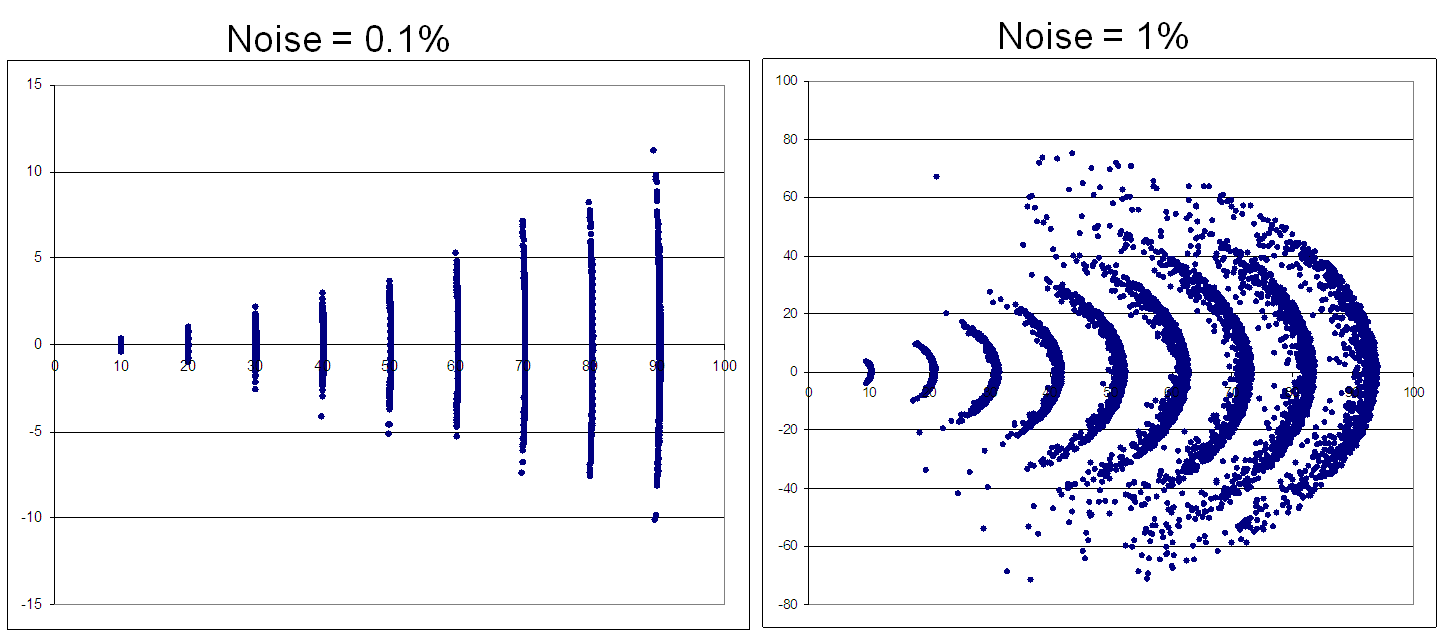
\includegraphics[width=0.7\linewidth]{deadreckoning1}
    \end{center}

\end{frame}

\begin{frame}{Dead reckoning: simulation (2)}

\begin{itemize}
    \item Robot taking a turn (left wheel speed = 1, right wheel speed = 1.005).
\end{itemize}

    \begin{center}
        \includegraphics[width=0.7\linewidth]{deadreckoning2}
    \end{center}
\end{frame}


\begin{frame}{}
    \begin{center}
        \Large
        That's all, folks!\\[2em]
        \normalsize
        Questions:\\
        Portland Square A216 or \url{severin.lemaignan@plymouth.ac.uk} \\[1em]

        Slides:\\ \href{https://github.com/severin-lemaignan/module-mobile-and-humanoid-robots}{\small github.com/severin-lemaignan/module-mobile-and-humanoid-robots}

    \end{center}
\end{frame}



\end{document}
